% ============================================================
% Final Project Presentation
% Project 05: Audiobook Generation (TTS Front-End)
% Course: CSC15012 - Applications of NLP in Industry
% Student: Le Dinh Minh Quan - 23127460 - 23CNTThuc
% Template based on Madrid + seahorse (Overleaf Beamer)
% ============================================================

\documentclass[10pt,aspectratio=169]{beamer}

\mode<presentation>
{
  \usetheme{Madrid}
  \usecolortheme{seahorse}
  \usefonttheme{default}
  \setbeamertemplate{navigation symbols}{}
  \setbeamertemplate{caption}[numbered]
  \setbeamertemplate{footline}[frame number]
}

% ---- Packages ----
\usepackage[english]{babel}
\usepackage[utf8]{inputenc}
\usepackage{amsmath}
\usepackage{graphicx}
\usepackage{booktabs}
\usepackage{xcolor}
\usepackage{hyperref}
\usepackage{xurl}
\usepackage{tikz}
\usepackage{pgfplots}
\pgfplotsset{compat=1.18}
\usetikzlibrary{shapes.geometric, arrows.meta, positioning, fit, backgrounds, shadows}
\usepackage{listings}
\lstset{
  basicstyle=\ttfamily\scriptsize,
  breaklines=true,
  frame=single,
  backgroundcolor=\color{gray!10},
  keywordstyle=\color{blue},
  commentstyle=\color{green!60!black},
  stringstyle=\color{red!70!black},
  showstringspaces=false,
  tabsize=2
}

% ---- HCMUS LOGO ----
% Upload logo_hcmus.png to Overleaf to display the logo (top-right of every slide).
% If the file is missing, no logo is shown (no error).
\IfFileExists{logo_hcmus.png}{\logo{\includegraphics[height=0.7cm]{logo_hcmus.png}}}{}

% ---- TITLE METADATA ----
\title[Project 05: Audiobook Generation]{Project 05: Audiobook Generation (TTS Front-End)}
\subtitle{A Trainable Text-Normalization Model with a Deterministic Agentic Pipeline}
\author[Le Dinh Minh Quan]{Le Dinh Minh Quan \\ \small ID: 23127460 -- Class: 23CNTThuc}
\institute[HCMUS]{Vietnam National University Ho Chi Minh City \\ University of Science -- Faculty of Information Technology \\ \small Course: CSC15012 -- Applications of NLP in Industry}
\date{2026}

\begin{document}

% ============================================================
% SLIDE 1: TITLE
% ============================================================
\begin{frame}
  \titlepage
\end{frame}

% ============================================================
% SLIDE 2: OUTLINE
% ============================================================
\begin{frame}{Outline}
\begin{columns}[T]
\begin{column}{0.5\textwidth}
\begin{enumerate}
  \item Business Problem \& Motivation
  \item Proposed NLP Solution \& Success Metrics
  \item System Architecture
  \item Repository \& Tech Stack
  \item Data Overview (synthetic TN corpus)
  \item Training \& Autopilot Workflow
  \item Evaluation: Baseline to Beat
\end{enumerate}
\end{column}
\begin{column}{0.5\textwidth}
\begin{enumerate}
  \setcounter{enumi}{7}
  \item Agentic AI Component (FSM, D1--D4)
  \item Agent Example Interaction
  \item Deployment (API / UI / CLI / Docker)
  \item Monitoring \& Continual Learning
  \item Privacy, Robustness \& Ethics
  \item Key Takeaways \& Future Work
  \item Resources \& Thank You
\end{enumerate}
\end{column}
\end{columns}
\end{frame}

% ============================================================
% SLIDE 3: BUSINESS PROBLEM & MOTIVATION
% ============================================================
\begin{frame}{1. Business Problem \& Motivation}
\begin{block}{Context}
Audiobook demand keeps rising, but human narration is slow and costly, and most text catalogs are never converted. Audiobook production fails on two NLP-heavy fronts: \textbf{text normalization} and \textbf{production orchestration}.
\end{block}

\begin{columns}[T]
\begin{column}{0.5\textwidth}
\textbf{Pain points}
\begin{itemize}
  \item Cost of studio narration per audio-hour
  \item Accessibility (sight-impaired, dyslexic, commuters)
  \item Scale: chaptering, chunking, voice routing, mastering
  \item Naive TTS mis-reads \texttt{\$5.2M}, \texttt{1984}, \texttt{Dr.}, \texttt{Chapter IV}
\end{itemize}
\end{column}
\begin{column}{0.5\textwidth}
\textbf{Stakeholders}
\begin{itemize}
  \item Readers with disabilities
  \item Commuters / language learners
  \item Independent authors
  \item Publishers (catalog conversion)
  \item Developers (REST API / CLI)
\end{itemize}
\end{column}
\end{columns}
\end{frame}

% ============================================================
% SLIDE 4: PROPOSED NLP SOLUTION + SUCCESS METRICS
% ============================================================
\begin{frame}{2. Proposed NLP Solution \& Success Metrics}
\begin{block}{Solution}
End-to-end \textbf{Audiobook Generator}: a trainable \textbf{ByT5-small Text-Normalization} model (written $\rightarrow$ spoken) + a pretrained \textbf{SpeechT5} TTS backend + a deterministic \textbf{agent FSM} (4 decisions) + a one-button Colab H100 autopilot.
\end{block}

\begin{table}[h]
\centering\small
\begin{tabular}{lll}
\toprule
\textbf{Type} & \textbf{Metric} & \textbf{Target} \\
\midrule
Business & Cost per finished audio-hour & $\ll$ human narration \\
Business & Unrecoverable mis-read rate / chapter & $\rightarrow 0$ \\
Technical & TN sentence EM \& macro per-class acc. & Beat the rule baseline \\
Technical & Loudness conformance & $-18$ LUFS / $-3$ dBTP (ACX) \\
Technical & Real-Time Factor (RTF) & $\sim$0.1 GPU; per-job \\
\bottomrule
\end{tabular}
\end{table}

\textbf{Verified offline:} rule baseline sentence EM = easy \textbf{0.945} / \textbf{hard 0.006} / overall \textbf{0.712} -- the bar the trained model must beat (especially on the hard slice). Validated agent run: \textbf{RTF 2.28} CPU, all 4 decisions fired, 0 flagged.
\end{frame}

% ============================================================
% SLIDE 5: SYSTEM ARCHITECTURE (TikZ)
% ============================================================
\begin{frame}{3. System Architecture (two-tier: CPU API + GPU worker)}
\centering
\resizebox{\linewidth}{!}{%
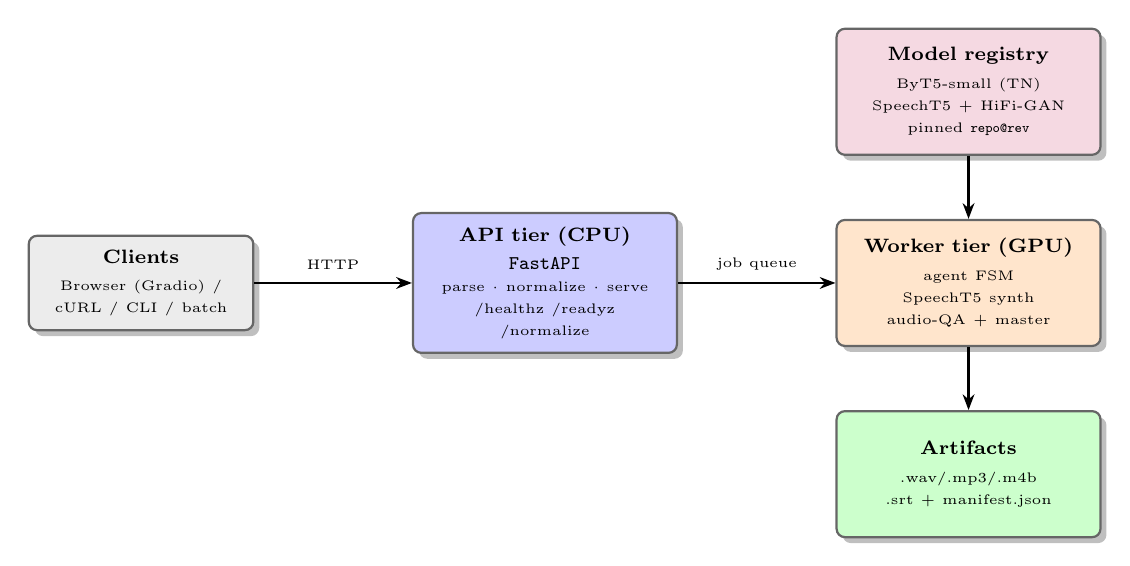
\begin{tikzpicture}[
  node distance=0.9cm and 2.0cm,
  box/.style={rectangle, draw=black!60, rounded corners=3pt, thick,
              text width=3.0cm, minimum height=1.6cm, align=center,
              inner sep=5pt, font=\scriptsize, drop shadow},
  clientbox/.style={box, fill=gray!15, text width=2.5cm, minimum height=1.0cm},
  apibox/.style={box, fill=blue!20},
  workerbox/.style={box, fill=orange!20},
  modelbox/.style={box, fill=purple!15},
  storebox/.style={box, fill=green!20},
  arrow/.style={-{Stealth[length=2mm]}, thick}
]

\node[clientbox] (client) {%
  \textbf{Clients}\\[2pt]
  {\tiny Browser (Gradio) / cURL / CLI / batch}
};
\node[apibox, right=of client] (api) {%
  \textbf{API tier (CPU)}\\[2pt]
  \texttt{FastAPI}\\
  {\tiny parse $\cdot$ normalize $\cdot$ serve}\\
  {\tiny /healthz /readyz /normalize}
};
\node[workerbox, right=of api] (worker) {%
  \textbf{Worker tier (GPU)}\\[2pt]
  {\tiny agent FSM}\\
  {\tiny SpeechT5 synth}\\
  {\tiny audio-QA + master}
};
\node[modelbox, above=0.8cm of worker] (models) {%
  \textbf{Model registry}\\[2pt]
  {\tiny ByT5-small (TN)}\\
  {\tiny SpeechT5 + HiFi-GAN}\\
  {\tiny pinned \texttt{repo@rev}}
};
\node[storebox, below=0.8cm of worker] (store) {%
  \textbf{Artifacts}\\[2pt]
  {\tiny .wav/.mp3/.m4b}\\
  {\tiny .srt + manifest.json}
};

\draw[arrow] (client.east) -- node[above=1pt, font=\tiny, midway] {HTTP} (api.west);
\draw[arrow] (api.east) -- node[above=1pt, font=\tiny, midway] {job queue} (worker.west);
\draw[arrow] (models.south) -- (worker.north);
\draw[arrow] (worker.south) -- (store.north);
\end{tikzpicture}%
}

\vspace{0.2cm}
\scriptsize \textbf{Separation of concerns}: a CPU API tier (parse/normalize/serve) is split from a GPU worker tier (agent + SpeechT5 + audio-QA + master) by a job queue, so synthesis scales by adding GPU workers. Every job writes a self-contained \texttt{manifest.json}.
\end{frame}

% ============================================================
% SLIDE 6: REPOSITORY & TECH STACK
% ============================================================
\begin{frame}[fragile]{4. Repository Structure \& Tech Stack}
\begin{columns}[T]
\begin{column}{0.55\textwidth}
\textbf{GitHub repo} (public, MIT) \\
\scriptsize \url{https://github.com/ledinhminhquan/05_Audiobook_Generation}

\vspace{0.15cm}
\begin{lstlisting}[basicstyle=\ttfamily\tiny]
05_Audiobook_Generation/
|-- src/audiobook_ai/
|   |-- data/        # tn_corpus.py (16 classes) + parsing
|   |-- models/      # baseline_rules + ByT5 + registry
|   |-- synthesis/   # SpeechT5 + stitch + subtitles
|   |-- training/    # Seq2SeqTrainer recipe + evaluate
|   |-- agent/       # FSM, D1-D4, tools, optional LLM
|   |-- api/         # FastAPI + Gradio UI + combined
|   |-- analysis/ autoreport/ monitoring/ grading/
|-- configs/  docs/(12)  tests/  sample_data/
|-- notebooks/        # Colab H100 AUTOPILOT
|-- deploy/           # Dockerfile (api/worker), compose
+-- Dockerfile  Makefile  pyproject.toml  README.md
\end{lstlisting}
\end{column}
\begin{column}{0.45\textwidth}
\textbf{Tech stack}
\begin{itemize}\small
  \item Python 3.12, Git + GitHub
  \item PyTorch, Transformers, \texttt{Seq2SeqTrainer}
  \item \textbf{ByT5-small} (TN, $\sim$300M, Apache-2.0)
  \item t5-small fallback; rule baseline (num2words)
  \item \textbf{SpeechT5} + HiFi-GAN (MIT)
  \item cmu-arctic x-vectors (7 speakers, MIT)
  \item ebooklib / PyMuPDF / pdfplumber / pysbd
  \item soundfile, pydub + ffmpeg, pyloudnorm, mutagen
  \item FastAPI + Uvicorn; Gradio (at \texttt{/ui})
  \item Docker (api CPU + worker GPU); HF Space
  \item Colab H100/A100/L4/T4 (auto-profiled)
\end{itemize}
\end{column}
\end{columns}
\end{frame}

% ============================================================
% SLIDE 7: DATA OVERVIEW
% ============================================================
\begin{frame}{5. Data Overview -- Synthetic TN Corpus}
\begin{columns}[T]
\begin{column}{0.5\textwidth}
\textbf{Why synthetic is PRIMARY}
\begin{itemize}\small
  \item No permissive English TN-Challenge mirror on HF Hub (\texttt{google/text\_normalization}, \texttt{cestwc/...} $\rightarrow$ 404)
  \item Deterministic generator $\Rightarrow$ any grader rebuilds the exact corpus, no downloads
  \item Optional VERIFIED sanity set: \texttt{DigitalUmuganda/...Eng\_Fra}
\end{itemize}

\textbf{Preprocessing}
\begin{itemize}\small
  \item Unicode NFC + task prefix \texttt{"normalize: "}
  \item Dedup before split; leakage-free
  \item PLAIN capped $\le$30\%
\end{itemize}
\end{column}
\begin{column}{0.5\textwidth}
\textbf{16 semiotic classes; injected ambiguity}
\begin{table}[h]
\centering\scriptsize
\begin{tabular}{ll}
\toprule
\textbf{Written} & \textbf{Context decides spoken} \\
\midrule
\texttt{St.} & Street \emph{vs} Saint \\
\texttt{1984} & year \emph{vs} count \\
\texttt{IV} & ``four'' (Roman) \emph{vs} ``I V'' \\
\bottomrule
\end{tabular}
\end{table}

\textbf{Default splits (English; $\approx$69.5k pairs)}
\begin{table}[h]
\centering\small
\begin{tabular}{lr}
\toprule
\textbf{Split} & \textbf{Size} \\
\midrule
train & 60,000 \\
val & 4,000 \\
test & 4,000 \\
hard (ambiguity stress) & \textbf{1,500} \\
\bottomrule
\end{tabular}
\end{table}
\end{column}
\end{columns}
\end{frame}

% ============================================================
% SLIDE 8: TRAINING / AUTOPILOT WORKFLOW
% ============================================================
\begin{frame}{6. Training \& Autopilot Workflow -- Colab H100}
\centering
\begin{tikzpicture}[
  node distance=0.18cm,
  step/.style={rectangle, draw=black!60, rounded corners=2pt, thick,
              minimum width=11.5cm, minimum height=0.5cm, align=center, font=\scriptsize},
  setup/.style={step, fill=gray!15},
  train/.style={step, fill=orange!15},
  eval/.style={step, fill=blue!15},
  deploy/.style={step, fill=green!15},
  arrow/.style={-{Stealth[length=1.8mm]}, thick}
]
\node[setup] (s1) {\textbf{1. Setup}: mount Drive, clone repo, install Colab-safe deps (never touch \texttt{torch})};
\node[setup, below=of s1] (s2) {\textbf{2. GPU auto-profile}: H100/A100/L4/T4 $\rightarrow$ batch + precision; effective batch held at \textbf{256}};
\node[setup, below=of s2] (s3) {\textbf{3. Build synthetic corpus}: 60k/4k/4k/1.5k (dedup, leakage-free, PLAIN $\le$30\%)};
\node[train, below=of s3] (s4) {\textbf{4. Train ByT5-small} (resume-safe): bf16+tf32, lr 5e-4, cosine, label smoothing 0.1, early stop};
\node[eval, below=of s4] (s5) {\textbf{5. Evaluate}: rule baseline vs.\ neural on \texttt{test}+\texttt{hard}; EM, macro/per-class, unrecoverable count};
\node[eval, below=of s5] (s6) {\textbf{6. Run agent FSM} on sample book: all 4 decisions fire; latency/RTF + audio-QA report};
\node[deploy, below=of s6] (s7) {\textbf{7. Auto-gen} report PDF + slides PPTX};
\node[deploy, below=of s7] (s8) {\textbf{8. Self-grade} + submission bundle (\texttt{audiobook-ai grade})};
\foreach \a/\b in {s1/s2,s2/s3,s3/s4,s4/s5,s5/s6,s6/s7,s7/s8}
  \draw[arrow] (\a) -- (\b);
\end{tikzpicture}

\vspace{0.12cm}
\scriptsize \textbf{One-button Run-All} on Colab H100. Auto-resume on disconnect; effective batch 256 across all GPUs; ByT5 $\approx$3--6\,h on one H100 (t5-small $\approx$3--4$\times$ faster, fits T4). CPU floor (\texttt{PlaceholderTTS}) keeps it testable with no weights.
\end{frame}

% ============================================================
% SLIDE 9: EVALUATION RESULTS
% ============================================================
\begin{frame}{7. Evaluation -- The Baseline to Beat}
\begin{columns}[T]
\begin{column}{0.5\textwidth}
\textbf{Validated rule-baseline EM} (synthetic \texttt{test})
\begin{table}[h]
\centering\small
\begin{tabular}{lc}
\toprule
\textbf{Slice} & \textbf{Sentence EM} \\
\midrule
Easy & 0.945 \\
\textbf{Hard (ambiguous)} & \textbf{0.006} \\
Overall & 0.712 \\
\bottomrule
\end{tabular}
\end{table}
\small The context-blind ruleset is near-perfect on easy inputs and \textbf{collapses on the hard slice (0.006)} -- honest, reproducible evidence that rules alone are insufficient.

\vspace{0.1cm}
\textbf{Metrics}: sentence EM (headline) $\cdot$ macro per-class accuracy (16 classes) $\cdot$ unrecoverable / ``silly'' error count $\rightarrow$0.
\end{column}
\begin{column}{0.5\textwidth}
\centering
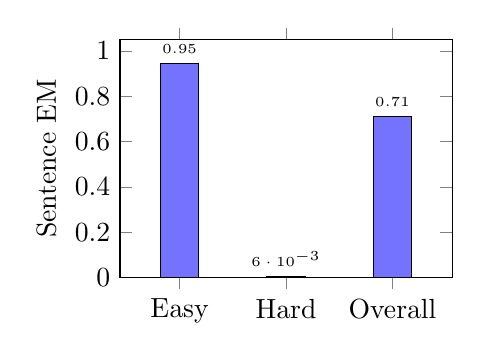
\begin{tikzpicture}
\begin{axis}[
  ybar, width=5.8cm, height=4.6cm,
  ymin=0, ymax=1.05,
  symbolic x coords={Easy, Hard, Overall},
  xtick=data,
  ylabel={Sentence EM},
  nodes near coords, every node near coord/.append style={font=\tiny},
  bar width=14pt,
  enlarge x limits=0.28,
  ytick={0,0.2,0.4,0.6,0.8,1.0}
]
\addplot[fill=blue!55] coordinates {(Easy,0.945) (Hard,0.006) (Overall,0.712)};
\end{axis}
\end{tikzpicture}\\
\tiny Rule baseline; the trained ByT5 is built to lift \textbf{hard} far above 0.006 while holding \textbf{easy}.
\end{column}
\end{columns}

\vspace{0.1cm}
\scriptsize \textbf{Offline vs.\ Colab}: the baseline + agent numbers are verified on the synthetic spine; the full ByT5 per-class table is produced by the Colab H100 autopilot. Expected win pattern: positive deltas concentrated in \texttt{ABBREV}, \texttt{ROMAN}, \texttt{DATE}, year-vs-count \texttt{CARDINAL}, \texttt{MONEY}, \texttt{TIME}.
\end{frame}

% ============================================================
% SLIDE 10: AGENTIC AI COMPONENT
% ============================================================
\begin{frame}{8. Agentic AI Component -- Deterministic FSM (D1--D4)}
\centering
\begin{tikzpicture}[
  node distance=0.18cm,
  step/.style={rectangle, draw=black!60, rounded corners=2pt, thick,
              text width=11.2cm, minimum height=0.5cm, align=center, font=\scriptsize,
              inner sep=4pt},
  parse/.style={step, fill=gray!15},
  seg/.style={step, fill=teal!15},
  norm/.style={step, fill=orange!15},
  voice/.style={step, fill=purple!12},
  synth/.style={step, fill=blue!15},
  qa/.style={step, fill=red!12},
  out/.style={step, fill=green!15},
  arrow/.style={-{Stealth[length=2mm]}, thick}
]
\node[parse] (p) {\textbf{1. PARSE + chapters} (tool) $\rightarrow$ \texttt{parse\_score} \quad \textbf{[D1]} structured / assisted / degraded};
\node[seg, below=of p] (s) {\textbf{2. SEGMENT + CLASSIFY} (tool): pysbd + chunk $\rightarrow$ narration\,|\,dialogue\,|\,heading\,|\,skip};
\node[norm, below=of s] (n) {\textbf{3. NORMALIZE} (tool + reasoning): ByT5 $\rightarrow$ spoken + conf \quad \textbf{[D2]} accept / flag / LLM / baseline};
\node[voice, below=of n] (v) {\textbf{4. VOICE-ROUTE} (decision) \quad \textbf{[D4]}: label $\rightarrow$ distinct x-vector, stable per book};
\node[synth, below=of v] (y) {\textbf{5a. SYNTHESIZE} (tool): SpeechT5 + HiFi-GAN, 16\,kHz, routed x-vector};
\node[qa, below=of y] (q) {\textbf{5b. AUDIO-QA} (decision) \quad \textbf{[D3]}: empty/NaN, duration, peak, silence $\rightarrow$ re-synth ($\le$2)};
\node[out, below=of q] (e) {\textbf{6. STITCH + EXPORT}: ACX $-18$ LUFS / $-3$ dBTP $\rightarrow$ wav/mp3/m4b + srt + manifest.json};
\foreach \a/\b in {p/s,s/n,n/v,v/y,y/q,q/e}
  \draw[arrow] (\a) -- (\b);
\end{tikzpicture}

\vspace{0.1cm}
\scriptsize Requires $\ge$3 decision points; \textbf{four delivered}. \textbf{Multi-step reasoning} (D2), \textbf{tool usage} (parse/normalize/route/synth/QA/stitch), \textbf{decision-making} on intermediate outputs (D1--D4). LLM brain consulted only at D2, validated, \textbf{off by default} (zero paid API).
\end{frame}

% ============================================================
% SLIDE 11: AGENT EXAMPLE INTERACTION
% ============================================================
\begin{frame}[fragile]{9. Agent Example Interaction (the sample book)}
\textbf{Hard NLP case: the written date ``March 3, 1921''}
\begin{lstlisting}[basicstyle=\ttfamily\tiny]
1) PARSE + D1: parse_score=0.93 >= 0.85 -> structured (3 chapters)
2) SEGMENT/CLASSIFY:
   "Chapter One"                                      -> heading
   "He returned on March 3, 1921, to an empty house." -> narration
   "\"You're late,\" she said."                       -> dialogue
3) NORMALIZE + D2: ByT5 ->
   "He returned on March third, nineteen twenty-one, to an empty house."
   (1921 read as YEAR; day 3 read as ORDINAL "third" -- context used) conf=0.88
   D2: 0.88 >= 0.55 -> ACCEPT (source=neural). 0 flagged.
4) VOICE-ROUTE + D4: heading/narration/dialogue -> 3 distinct x-vectors (fixed/book)
5) SYNTHESIZE + AUDIO-QA + D3: SpeechT5 renders; clip says "nineteen twenty-one";
   all clips PASS attempt 1 -> accept (no re-synth)
6) STITCH + EXPORT: ACX -18 LUFS / -3 dBTP -> wav/mp3/m4b + srt + manifest
   (input_sha256, 3 chapters, sources/confidences, 4 Decisions, 0 flags, RTF 2.28)
\end{lstlisting}

\scriptsize A context-blind baseline would risk ``March three, one thousand nine hundred twenty-one'' -- exactly the failure the trained context-aware normalizer fixes. \textbf{Every decision fired; no human intervention; no paid API.}
\end{frame}

% ============================================================
% SLIDE 12: DEPLOYMENT
% ============================================================
\begin{frame}{10. Deployment -- Four Surfaces over One Core}
\textbf{Deployment formats delivered (4 of 4 possible types)}
\begin{itemize}\small
  \item \textbf{REST API} (FastAPI): \texttt{/healthz} \texttt{/readyz} \texttt{/normalize} \texttt{/synthesize} \texttt{/synthesize/file} \texttt{/download}
  \item \textbf{Gradio web demo}: mounted at \texttt{/ui}; published as a CPU-only HF Space
  \item \textbf{CLI} (\texttt{audiobook-ai}): \texttt{data/train/evaluate/normalize/synthesize/demo-agent/serve/autopilot/grade}
  \item \textbf{Batch}: same pipeline over a directory; each job a self-contained \texttt{manifest.json}
\end{itemize}

\begin{columns}[T]
\begin{column}{0.5\textwidth}
\textbf{Latency (RTF)} -- validated run
\begin{table}[h]
\centering\small
\begin{tabular}{ll}
\toprule
\textbf{Env} & \textbf{RTF} \\
\midrule
CPU (validated) & \textbf{2.28} \\
GPU (estimated) & $\sim$0.1 \\
\bottomrule
\end{tabular}
\end{table}
\scriptsize 3 chapters, 7 segments, 0 flagged, 67\,s WAV + SRT + manifest.
\end{column}
\begin{column}{0.5\textwidth}
\textbf{Scalability \& versioning}
\begin{itemize}\scriptsize
  \item Chunk-level parallelism + GPU micro-batching
  \item Queue-based API(CPU)/worker(GPU) split
  \item Time-to-first-audio: stream chapter 1
  \item Registry pins \texttt{repo@revision}; commercial path MIT/Apache only
  \item Docker (api/worker) + HF Space (CPU)
\end{itemize}
\end{column}
\end{columns}

\vspace{0.1cm}
\scriptsize \textit{Status}: deployable and CPU-only with zero paid API; not currently hosted at a fixed public URL.
\end{frame}

% ============================================================
% SLIDE 13: MONITORING & CONTINUAL LEARNING
% ============================================================
\begin{frame}{11. Monitoring \& Continual Learning}
\begin{columns}[T]
\begin{column}{0.5\textwidth}
\textbf{Monitoring} (\texttt{drift\_report.py})
\begin{itemize}\small
  \item \textbf{TN flag-rate} (D2 conf $<$0.55 / disagreement) -- $\uparrow$ bad
  \item \textbf{Audio-QA fail-rate} (D3) -- $\uparrow$ bad
  \item \textbf{RTF drift} ($\sim$2.28 CPU / $\sim$0.1 GPU) -- $\uparrow$ bad
  \item \textbf{Confidence histogram} -- left-shift bad
  \item \textbf{Per-class golden-set accuracy} -- $\downarrow$ bad
\end{itemize}
\scriptsize Diffed against fixed anchors: golden set, shipped test/hard slices, incumbent model.
\end{column}
\begin{column}{0.5\textwidth}
\textbf{Continual learning loop}
\begin{enumerate}\small
  \item Collect D2/D3 flags + user corrections (gold labels)
  \item Augmented corpus = regenerated synthetic + real corrections + sanity set
  \item Fine-tune (lr 5e-4, eff.\ batch 256, early stop)
  \item Offline gate: beat test + hard, no macro-class regression
  \item Canary $\rightarrow$ A/B behind \texttt{latest} pointer
  \item Promote or roll back (one-line \texttt{repo@rev} change)
\end{enumerate}
\end{column}
\end{columns}

\vspace{0.15cm}
\centering
\scriptsize The loop is circular: \textbf{flags $\rightarrow$ feedback store $\rightarrow$ augmented corpus $\rightarrow$ periodic fine-tune $\rightarrow$ registry-versioned canary/AB $\rightarrow$ drift monitoring $\rightarrow$ new flags}, so accuracy on the \emph{served} distribution improves over time.
\end{frame}

% ============================================================
% SLIDE 14: PRIVACY, ROBUSTNESS & ETHICS
% ============================================================
\begin{frame}{12. Privacy, Robustness \& Ethics}
\begin{columns}[T]
\begin{column}{0.5\textwidth}
\textbf{Privacy} (PII in TELEPHONE/ELECTRONIC/ABBREV)
\begin{itemize}\scriptsize
  \item Logs carry metrics/decisions, \textbf{not raw text}
  \item NER for D4 attribution only, then discarded
  \item TTL cleanup; optional redaction/skip
  \item Input SHA-256 recorded (rights/provenance)
\end{itemize}

\textbf{Robustness}
\begin{itemize}\scriptsize
  \item Byte-level ByT5 = robust to numbers/symbols/OOV
  \item OOD (scanned PDF / OCR) $\rightarrow$ low \texttt{parse\_score} $\rightarrow$ degraded path (D1)
  \item Guardrail (rules) + D3 QA gate + unrecoverable count
  \item Backend ladder ends at \texttt{PlaceholderTTS} $\Rightarrow$ never hard-fails
\end{itemize}
\end{column}
\begin{column}{0.5\textwidth}
\textbf{Ethics \& fairness (named, not hidden)}
\begin{itemize}\scriptsize
  \item \textbf{Voice coverage narrow}: 7 default speakers
  \item \textbf{English-/US-centric} normalization conventions
  \item \textbf{Name pronunciation} may be subtly wrong
  \item \textbf{Labor displacement} of human narrators
\end{itemize}

\textbf{Safeguards}
\begin{itemize}\scriptsize
  \item Voice-cloning (XTTS / F5 / MMS) \textbf{non-commercial, consent-gated, OFF by default}
  \item Commercial path = MIT/Apache only (license hygiene)
  \item Auditable: per-segment script + D1--D4 log + manifest
  \item Non-deceptive degradation (a degraded run is flagged)
\end{itemize}
\end{column}
\end{columns}
\end{frame}

% ============================================================
% SLIDE 15: KEY TAKEAWAYS & FUTURE WORK
% ============================================================
\begin{frame}{13. Key Takeaways \& Future Work}
\textbf{Key takeaways}
\begin{itemize}\small
  \item Complete end-to-end NLP system: corpus $\rightarrow$ training $\rightarrow$ evaluation $\rightarrow$ agent $\rightarrow$ deployment $\rightarrow$ monitoring
  \item Trainable core = \textbf{ByT5-small} byte-level TN (OOV-free, char-faithful) with a context-blind rule baseline to beat (\textbf{easy 0.945 / hard 0.006 / overall 0.712} EM, verified offline)
  \item Deterministic \textbf{agent FSM} with \textbf{4 decisions} (D1--D4): reasoning + tools + decision-making; validated end-to-end (\textbf{RTF 2.28} CPU, all 4 fired, 0 flagged)
  \item \textbf{Deployable} 4 ways (REST API + Gradio UI + CLI + batch) + Docker + HF Space, CPU-only, zero paid API; ACX $-18$ LUFS / $-3$ dBTP
  \item License-clean by design: commercial path MIT/Apache only; non-commercial cloning flagged + gated off
\end{itemize}

\textbf{Future work}
\begin{enumerate}\small
  \item Scale-up data: convert the off-Hub Google TN Challenge ($\sim$1.1B words, 16 classes)
  \item Quality TTS behind a toggle: Kokoro (24\,kHz) / prompt-styled Parler voices
  \item Word-level forced-aligned \texttt{.srt} timestamps (permissive aligner)
  \item Consent-gated character voices (research/demo only)
  \item Drift dashboard over \texttt{manifest.json} + canary A/B rollout
\end{enumerate}
\end{frame}

% ============================================================
% SLIDE 16: RESOURCES & THANK YOU (Final slide)
% ============================================================
\begin{frame}{14. Project Resources \& Thank You}
\begin{block}{Source code (public, MIT)}
\centering
\large \textbf{\url{https://github.com/ledinhminhquan/05_Audiobook_Generation}}
\end{block}

\textbf{Resources}
\begin{itemize}\scriptsize
  \item \textbf{GitHub repo}: \url{https://github.com/ledinhminhquan/05_Audiobook_Generation}
  \item \textbf{Reference inspiration}: \texttt{denizsafak/abogen} -- \url{https://github.com/denizsafak/abogen}
  \item \textbf{Deployment}: FastAPI REST API + Gradio UI + CLI + batch + Docker + HF Space (CPU-only, zero paid API)
  \item \textbf{Training}: one-button Colab H100 autopilot notebook (\texttt{notebooks/}) -- auto-profiles H100/A100/L4/T4
  \item \textbf{Models}: \texttt{google/byt5-small} (Apache-2.0) + \texttt{microsoft/speecht5\_tts} + HiFi-GAN (MIT) + cmu-arctic x-vectors (MIT)
\end{itemize}

\vspace{0.3cm}
\centering
\Large\textbf{Thank you for your attention!}\\[0.2cm]
\normalsize Le Dinh Minh Quan -- 23127460 -- 23CNTThuc \\
\small CSC15012 -- Applications of NLP in Industry -- 2026
\end{frame}

\end{document}
